\graphicspath{{04_ODEs/figures/PNG/}{04_ODEs/figures/PDF/}{04_ODEs/figures/}}


\chapter{Introduzione alle ODEs (e sistemi di ODEs) non lineari}
\copyrightnotice
\section{Cenni sugli spazi metrici}
\begin{definition}
\mbox{}
\begin{enumerate}[labelindent=\parindent,leftmargin=*,label=\textnormal{(\roman*)},start=1]
\item Dato un insieme $X$, si chiama \emph{metrica su $X$} una funzione $\mathrm{d} : X \times X \longrightarrow [0,\,+\infty]$ verificante
	\begin{enumerate}[labelindent=\parindent,leftmargin=*,label=\textnormal{(d\arabic*)},start=1]
	\item $\mathrm{d}(x,\,y) = 0 \quad\Longleftrightarrow\quad x=y$
	\item $\mathrm{d}(x,\,y) = \mathrm{d}(y,\,x) \qquad \forall \, x,\,y \in X$
	\item $\mathrm{d}(x,\,y) \leq \mathrm{d}(x,\,z) + \mathrm{d}(z,\,y) \qquad \forall x,\,y,\,z \in X$
	\end{enumerate}
\item Una successione $(x_n)_n \subset X$ si dice convergente in $(X,\,\mathrm{d})$ se $\exists \, x \in X$ tale che
$$
\lim_{h \rightarrow \infty} \mathrm{d}(x_h,\,x) = 0
$$
\item Una successione $(x_n)_n \subset X$ si dice una \emph{successione di Cauchy} se $\forall \, \varepsilon > 0 \quad \exists \, \overline{h} = \overline{h}(\varepsilon) \in \mathbb{N}$ tale che
$$
\mathrm{d}(x_h,\,x_k) < \varepsilon \qquad \forall h,\,k > \overline{h}
$$
\item Uno spazio metrico $(X,\,\mathrm{d})$ si dice \emph{completo} se ogni successione di Cauchy $(x_n)_n \subset X$ è convergente, cioè $\exists \, x \in X$ tale che
$$
\exists \, \lim_{h \rightarrow \infty} \mathrm{d}(x_h,\,x) = 0
$$
\item Siano $(X,\,\mathrm{d})$ e $(Y,\,\mathrm{p})$ spazi metrici e sia $T : X \longrightarrow Y$. $T$ si dice \emph{continua} (su $X$) se, data $(x_n)_n \subset X$ con $\; \displaystyle \lim_{h \rightarrow \infty} x_h = x \quad (\text{in } X) \quad\Longrightarrow\quad \lim_{h \rightarrow \infty} T(x_h) = T(x) \quad (\text{in } Y)$.
\end{enumerate}
\end{definition}


\begin{thm}[delle contrazioni o del punto fisso, di \textsc{Banach - Caccioppoli}]
Sia $(X,\,\mathrm{d})$ uno spazio metrico completo e sia $T : X \longrightarrow X$. Supponiamo che $T$ sia una contrazione, cioè $\exists \, \alpha \in (0,\,1)$ tale che
\begin{center}
$\mathrm{(C)}$
\hfill
$\displaystyle
\mathrm{d}\left( T(x),\,T(y) \right) \leq \alpha \cdot \mathrm{d}(x,\,y) \qquad \forall \, x,\,y \in X
$
\hfill \null \\
\end{center}
Allora esiste un \emph{unico punto fisso} $\overline{x} \in X$ tale che $T(\overline{x}) = \overline{x}$.
\end{thm}
\begin{proof}
Dimostriamo prima l'unicità e poi l'esistenza.

\noindent\underline{Unicità}\\
Supponiamo per assurdo che esistano due punti fissi $\overline{x},\,x^* \in X$ tali che $\overline{x} \neq x^*$ e
\begin{center}
$\mathrm{(1)}$
\hfill
$\displaystyle
T(\overline{x}) = \overline{x}
$
\hfill \null \\
\vskip 10pt
$\mathrm{(2)}$
\hfill
$\displaystyle
T(x^*) = x^*
$
\hfill \null \\
\end{center}
Dalla $\mathrm{(C)}$, abbiamo che
$$
\underline{\mathrm{d}(x^*,\,\overline{x})} \overset{\mathrm{(1)}+\mathrm{(2)}}{=}
\mathrm{d}\left( T(x^*),\,T(\overline{x}) \right) \leq
\underline{\alpha \cdot \mathrm{d}(x^*,\,\overline{x})}
$$
da cui segue che
$$
(1-\alpha) \cdot \mathrm{d}(x^*,\,\overline{x}) \leq 0
$$
Poiché $\alpha \neq 1$ e, in particolare, $\alpha < 1$, possiamo dividere ambo i membri della disuguaglianza per $(1-\alpha) > 0$, ottenendo
$$
\mathrm{d}(x^*,\,\overline{x}) \leq 0
$$
Ma $\mathrm{d} \geq 0$ per definizione, quindi in definitiva
$$
\mathrm{d}(x^*,\,\overline{x}) = 0
$$
Utilizzando la proprietà $\mathrm{(d1)}$, ne segue che $x^* = \overline{x}$, assurdo per le ipotesi fatte. Questo prova la tesi.

\noindent\underline{Esistenza}\\
Fissiamo $x_0 \in X$ e definiamo una successione $(x_h)_h \in X$ per ricorrenza nel modo seguente:
$$
\begin{array}{lcr}
x_0 \doteqdot x_0 & \qquad & \text{per } h=0\\
x_1 \doteqdot T(x_0) & \qquad & \text{per } h=1\\
x_2 \doteqdot T(x_1) & \qquad & \text{per } h=2\\
\vdots & & \\
x_{h+1} \doteqdot T(x_h) & \qquad & (\star)\\
\end{array}
$$
Proviamo che $(x_h)_h$ è convergente, cioè $\exists \, \overline{x} \in X$ tale che
\begin{center}
$\mathrm{(1)}$
\hfill
$\displaystyle
\exists \, \lim_{h \rightarrow \infty} x_h = \overline{x} \qquad\qquad (\text{in } X)
$
\hfill \null \\
\end{center}
Per provare la $\mathrm{(1)}$, basta provare che $(x_h)_h$ è una successione di Cauchy\footnote{Infatti, in uno spazio metrico \emph{completo}, una successione è convergente se e solo se è di Cauchy.} in $(X,\,\mathrm{d})$, cioè $\forall \, \varepsilon > 0 \quad \exists \, \overline{h}$ tale che
$$
\mathrm{d}(x_h,\,x_k) < \varepsilon \qquad \forall h,\,k > \overline{h}
$$
Osserviamo che
$$
\begin{array}{rl}
\underline{\mathrm{d}(x_{h+1},\,x_h)} \overset{\mathrm{(\star)}}{=} & 
\mathrm{d}\left( T(x_h),\,T(x_{h-1}) \right) \overset{\mathrm{(C)}}{\leq}
\alpha \cdot \mathrm{d}(x_h,\,x_{h-1}) =\\
& = \alpha \cdot \mathrm{d}\left( T(x_{h-1}),\,T(x_{h-2}) \right) \leq
\alpha^2 \cdot \mathrm{d}(x_{h-1},\,x_{h-2}) =\\
& = \ldots//\ldots \leq \underline{\alpha^h \cdot \mathrm{d}(x_1,\,x_0)}
\end{array}
$$
ossia
\begin{center}
$\mathrm{(2)}$
\hfill
$\displaystyle
\mathrm{d}(x_{h+1},\,x_h) \leq \alpha^h \cdot \mathrm{d}(x_1,\,x_0) \qquad \forall \, h \in \mathbb{N}
$
\hfill \null \\
\end{center}
Siano $k,\,h \in \mathbb{N}, \quad k < h$. Vale
$$
\mathrm{d}(x_k,\,x_h) \overset{\mathrm{(d3)}}{\leq} 
\sum_{i=k}^{h-1} \mathrm{d}(x_{i+1},\,x_i) \overset{\mathrm{(2)}}{\leq}
\sum_{i=k}^{h-1} \alpha^i \cdot \mathrm{d}(x_1,\,x_0) =
\mathrm{d}(x_1,\,x_0) \sum_{i=k}^{h-1} \alpha^i \overset{\footnotemark}{=}
$$
\footnotetext{\`E una serie geometrica.}
$$
= \mathrm{d}(x_1,\,x_0) \dfrac{\alpha^{k}-\alpha^h}{1-\alpha} \leq
\mathrm{d}(x_1,\,x_0) \dfrac{\alpha^{k}}{1-\alpha}
$$
Dunque abbiamo provato che
\begin{center}
$\mathrm{(3)}$
\hfill
$\displaystyle
\mathrm{d}(x_k,\,x_h) \leq \frac{\mathrm{d}(x_1,\,x_0)}{1-\alpha} \alpha^{k} \underset{k \rightarrow \infty}{\longrightarrow} 0 \qquad \forall \, h > k
$
\hfill \null \\
\end{center}
Quindi, $\forall \, \varepsilon > 0 \quad \exists \, \overline{h} = \overline{h}(\varepsilon)$ tale che 
%Facendo tendere $k \rightarrow \infty$, segue che
\begin{center}
$\mathrm{(4)}$
\hfill
$\displaystyle
\mathrm{d}(x_k,\,x_h) < \varepsilon \qquad \forall \, h>k>\overline{h}
$
\hfill \null \\
\end{center}
o, in altre parole, $\forall \, \varepsilon > 0$ riusciamo sempre a trovare il più piccolo $\overline{h}$ (perché $\frac{\mathrm{d}(x_1,\,x_0)}{1-\alpha} \alpha^{k} \underset{k \rightarrow \infty}{\longrightarrow} 0$) per cui
$$
\mathrm{d}(x_{\overline{h}},\,x_h) \leq \frac{\mathrm{d}(x_1,\,x_0)}{1-\alpha} \alpha^{\overline{h}} < \varepsilon
$$
e di conseguenza prendendo qualsiasi $h>k>\overline{h}$, si verifica la $\mathrm{(4)}$.

Avendo provato la $\mathrm{(1)}$, proviamo che $\overline{x}$ è un punto fisso di $T$ per completare la dimostrazione. Da $\mathrm{(1)}$ segue che anche la successione $(x_{h+1})_h$ è convergente a $\overline{x} \in X$, poiché è una successione estratta da $(x_h)_h$. Inoltre, poiché $T$ è lipschitziana con costante di Lipschitz $\alpha < 1$ e ogni funzione lipschitziana è continua, $T$ è continua. D'altra parte, dalla $\mathrm{(\star)}$ segue che (utilizzando la continuità di $T$):
$$
\begin{array}{ccc}
x_{h+1} &=& T(x_h)\\
\rotatebox{270}{$\longrightarrow$} & & \rotatebox{270}{$\longrightarrow$}\\
\overline{x} &=& T(\overline{x})\\
\end{array}
$$
\end{proof}

Con l'idea di applicare il Teorema del punto fisso allo spazio di funzioni $C^0([a,\,b])$, consideriamo il seguente lemma.

\begin{lemma} \label{lemma_metrici} 
\mbox{}
\begin{enumerate}[labelindent=\parindent,leftmargin=*,label=\textnormal{(\roman*)},start=1]
\item Sia $f \in C^0([a,\,b])$ con $a,\,b \in \mathbb{R}, \; \; a<b$, e definiamo
$$
||f||_{\infty} \doteqdot \underset{x \in [a,\,b]}{\max} |f(x)| \in [0,\,+\infty)
$$
(esiste per il teorema di Weierstrass). Allora $||\cdot||_{\infty}$ è una \emph{norma} in $C^0([a,\,b])$.
\item Siano $f,\,g \in C^0([a,\,b])$. Definiamo
$$
\mathrm{d}(f,\,g) \doteqdot ||f-g||_{\infty}
$$
Allora $\left( C^0([a,\,b]),\,\mathrm{d} \right)$ è uno spazio metrico \emph{completo}.
\end{enumerate}
\end{lemma}
\begin{proof}
\begin{enumerate}[labelindent=\parindent,leftmargin=*,label=\textnormal{(\roman*)},start=1]
\item Le proprietà
	\begin{enumerate}[labelindent=\parindent,leftmargin=*,label=\textnormal{(N\arabic*)},start=1]
	\item $||f||_{\infty} = 0 \quad\Longleftrightarrow\quad f \equiv 0$ su $[a,\,b]$
	\item $||\lambda f||_{\infty} = |\lambda| \cdot ||f||_{\infty} \qquad \forall \, f,\,g \in C^0([a,\,b])$
	\end{enumerate}
sono banali. La proprietà
	\begin{enumerate}[labelindent=\parindent,leftmargin=*,label=\textnormal{(N\arabic*)},start=3]
	\item $||f+g||_{\infty} \leq ||f||_{\infty} + ||g||_{\infty} \qquad \, f,\,g \in C^0([a,\,b])$
	\end{enumerate}
discende dalla disuguaglianza triangolare per la norma $|\cdot|$ in $\mathbb{R}$.

\item Dobbiamo provare che, data $(f_h)_h \subset \left( C^0([a,\,b]),\,\mathrm{d}_{\infty} \right)$ successione di Cauchy, esiste $f \in C^0([a,\,b])$ tale che
$$
\lim_{h \rightarrow \infty} \mathrm{d}_{\infty} (f_h,\,f) \doteqdot \lim_{h \rightarrow \infty} ||f_h-f||_{\infty} = 0
$$
Per ipotesi $(f_h)_h$ è di Cauchy, cioè $\forall \, \varepsilon > 0 \quad \exists \, \overline{h} = \overline{h}(\varepsilon) \in \mathbb{N}$ tale che
\begin{center}
$\mathrm{(1)}$
\hfill
$\displaystyle
||f_h-f_k||_{\infty} < \varepsilon \qquad \forall \, k > h > \overline{h}
$
\hfill \null \\
\end{center}
Dalla $\mathrm{(1)}$ e dalla definizione di norma a $\infty$, segue che $\forall \, \varepsilon > 0 \quad \exists \, \overline{h} = \overline{h}(\varepsilon) \in \mathbb{N}$ tale che
\begin{center}
$\mathrm{(2)}$
\hfill
$\displaystyle
\left| f_h(t)-f_k(t) \right| < \varepsilon \qquad \forall \, k > h > \overline{h}, \quad \forall \, t \in [a,\,b]\footnotemark
$
\hfill \null \\
\end{center}
\footnotetext{
Dalla definizione otteniamo in realtà che $\underset{t \in [a,\,b]}{\max} \left| f_h(t)-f_k(t) \right| < \varepsilon$. Ma se tale proprietà vale per il massimo, allora vale anche per ogni $t$.
}
Fissiamo $t \in [a,\,b]$ e consideriamo la successione $(f_h(t))_h \subset (\mathbb{R},\,|\cdot|)$. Dalla $\mathrm{(2)}$ discende che $(f_h(t))_h$ è una successione di Cauchy in $(\mathbb{R},\,|\cdot|)$, che sappiamo essere uno spazio metrico completo. Dunque (poiché ogni successione di Cauchy è convergente in uno spazio metrico completo),
$$
\exists \, \lim_{h \rightarrow \infty} f_h(t) \doteqdot f(t) \qquad (\text{in } \mathbb{R})
$$
Abbiamo quindi costruito una funzione $f: [a,\,b] \longrightarrow \mathbb{R}$ tale che
$$
f(t) \doteqdot \lim_{h \rightarrow \infty} f_h(t) \qquad (\text{in } \mathbb{R})
$$
Per concludere, basta provare che
\begin{center}
$\mathrm{(3)}$
\hfill
$\displaystyle
f \in C^0([a,\,b])
$
\hfill \null \vskip 0pt
$\mathrm{(4)}$
\hfill
$\displaystyle
||f_h-f||_{\infty} \underset{h \rightarrow \infty}{\longrightarrow} 0
$
\hfill \null \\
\end{center}
Fissiamo $h$ nella $\mathrm{(2)}$ e facciamo tendere $k \rightarrow \infty$, ottenendo che $\forall \varepsilon > 0 \quad \exists \, \overline{h} = \overline{h}(\varepsilon) \in \mathbb{N}$ tale che
\begin{center}
$\mathrm{(5)}$
\hfill
$\displaystyle
\left| f_h(t)-f(t) \right| \leq \varepsilon \qquad \forall \, h > \overline{h}, \quad \forall \, t \in [a,\,b]
$
\hfill \null \\
\end{center}
In altre parole, $f$ è uniformemente\footnote{Nel senso che $h$ non dipende da $t$.} vicina ad una funzione $f_h$ continua per ipotesi. Proviamo ora che, fissato $t_0 \in [a,\,b]$, $f$ è continua in $t_0$, cioè
$$
\exists \, \lim_{t \rightarrow t_0} f(t) = f(t_0)
$$
Fissati $t,\,t_0 \in [a,\,b]$, $\forall \, h \in \mathbb{N}$ vale che
\begin{center}
$\mathrm{(6)}$
\hfill
$\displaystyle
|f(t)-f(t_0)| = 
\left| \big(f(t)-f_h(t)\big)+\big(f_h(t)-f_h(t_0)\big)+\big(f_h(t_0)-f(t_0)\big) \right| \leq
|f(t)-f_h(t)| + |f_h(t)-f_h(t_0)| + |f_h(t_0)-f(t_0)|
$
\hfill \null \\
\end{center}
Dalla $\mathrm{(5)}$ e dalla $\mathrm{(6)}$ segue che, fissato $\varepsilon > 0, \; \exists \, \overline{h} = \overline{h}(\varepsilon)$ tale che
\begin{center}
$\mathrm{(7)}$
\hfill
$\displaystyle
|f(t)-f(t_0)| \leq 2\varepsilon + |f_h(t)-f_h(t_0)| \qquad \forall \, h > \overline{h}, \quad \forall \, t,\,t_0 \in [a,\,b]
$
\hfill \null \\
\end{center}
Scegliendo $h^* = \overline{h}+1$, dalla continuità di $f_{h^*}$ in $t_0$ segue che, $\forall \, \varepsilon > 0, \; \exists \, \delta_0 > 0$ tale che
\begin{center}
$\mathrm{(8)}$
\hfill
$\displaystyle
|f_{h^*}(t)-f_{h^*}(t_0)| < \varepsilon \qquad \forall \, t \in (t_0-\delta_0,\,t_0+\delta_0) \cap [a,\,b]
$
\hfill \null \\
\end{center}
Da $\mathrm{(7)}+\mathrm{(8)}$, concludiamo che $\forall \, t_0 \in [a,\,b], \; \forall \varepsilon > 0 \quad \exists \delta_0 = \delta_0(\varepsilon,\,t_0) > 0$ tale che
\begin{center}
$ \displaystyle
|f(t) - f(t_0)| \leq 3\varepsilon \qquad \forall \, t \in (t_0-\delta_0,\,t_0+\delta_0) \cap [a,\,b]
$\\
$ \displaystyle
\rotatebox{270}{$\overset{\rotatebox{90}{\footnotesize \textit{def}}}{\Longleftrightarrow}$}
$\\
$$
\exists \, \lim_{t \rightarrow t_0} f(t) = f(t_0)
$$
\end{center}
La proprietà $\mathrm{(4)}$ segue banalmente dalla $\mathrm{(5)}$.
\end{enumerate}
\end{proof}

\begin{obs} In $\left( C^0([a,\,b]),\,\mathrm{d} \right)$ fallisce la proprietà che, data $(f_h)_h$ una successione limitata, esiste una sua sottosuccessione convergente (teorema di Bolzano-Weierstrass).
\end{obs}



\section{ODEs}
\begin{example}[\RNum{2} Legge della Dinamica di Newton]
La \RNum{2} Legge della Dinamica è spesso espressa nella forma
\begin{center}
$\mathrm{(\RNum{2}LN)}$
\hfill
$\displaystyle
\underline{F} = m \underline{a}
$
\hfill \null \\
\end{center}
Tuttavia, è possibile anche una sua formalizzazione tramite le ODEs\footnote{``ODE(s)'' = ``Ordinary Differential Equation(s)'', abbreviate anche ``EDO'' in italiano (``Equazioni Differenziali Ordinarie'')}:
$$
x = x(t) \qquad\Longrightarrow\qquad \overset{..}{x} = \frac{\partial^2 x}{\partial t^2}
\qquad\Longrightarrow\qquad F(t,\,x,\,\overset{.}{x}) = m \overset{..}{x}
$$
In $\mathbb{R}^3$, $x(t) = (x_1(t),\,x_1(t),\,x_3(t))$ descrive il vettore posizione di un punto materiale di massa $m$, mentre $\underline{F} : \mathbb{R}^3 \longrightarrow \mathbb{R}^3$ è la forza applicata al punto stesso. Se ad un certo istante $t_0 \quad x(t_0) = P_0$, qual'è l'espressione di $x(t) \quad (t>t_0)$?

In tal caso, $\mathrm{(\RNum{2}LN)}$ è equivalente al sistema di $3$ ODEs in $3$ incognite
$$
\begin{cases}
m \overset{..}{x_1} = F_1(t,\,x,\,\overset{.}{x})\\
m \overset{..}{x_2} = F_2(t,\,x,\,\overset{.}{x})\\
m \overset{..}{x_3} = F_3(t,\,x,\,\overset{.}{x})\\
\end{cases}
$$
\end{example}

Restringiamoci, per il momento, allo studio di un'equazione differenziale ordinaria di ordine $n$ in forma \emph{normale}, cioè
\begin{center}
$\mathrm{(E)}$
\hfill
$\displaystyle
x^{(n)} = f \left( t,\,x,\,x',\ldots,x^{n-1} \right)
$
\hfill \null \\
\end{center}
dove $f : A \subseteq \mathbb{R}^{n+1} \longrightarrow \mathbb{R}$ continua, $A$ aperto, $x : I \longrightarrow \mathbb{R}$, $I$ intervallo di $\mathbb{R}$.

\begin{example}[Equazione del pendolo]
L'equazione del pendolo semplice è un'equazione del secondo ordine non lineare, nella forma
$$
\overset{..}{\vartheta} = - \omega^2 \sin(\vartheta)
$$
La sua soluzione - ovviamente - non è banale a causa della non linearità.
\end{example}

\begin{definition}[di soluzione di $\mathrm{(E)}$]
Si chiama \emph{soluzione di $\mathrm{(E)}$} una funzione $x = x(t) \in C^n(I)$ dove $I \subseteq \mathbb{R}$ è un \emph{intervallo} tale che
\begin{enumerate}[labelindent=\parindent,leftmargin=*,label=\textnormal{(S$_\arabic*$)},start=1]
\item $\left( t,\,x(t),\,x'(t),\ldots,x^{n-1}(t) \right) \in A \qquad \forall t \in I$
\item $x^{(n)}(t) = f \left( t,\,x(t),\,x'(t),\ldots,x^{n-1}(t) \right) \qquad \forall t \in I$
\end{enumerate}
Una soluzione di $\mathrm{(E)}$ si dice anche \emph{curva integrale di $\mathrm{(E)}$}.
\end{definition}

\noindent\underline{Problema:} determinare l'integrale generale di $\mathrm{(E)}$, cioè l'insieme delle soluzioni di $\mathrm{(E)}$.

\subsection{Caso $n=1$}
Restringiamoci per il momento alle ODEs del \RNum{1} ordine, ossia consideriamo il caso $n=1$. L'equazione $\mathrm{(E)}$ si riduce a
\begin{center}
$\mathrm{(E)}$
\hfill
$\displaystyle
x' = f \left( t,\,x \right)
$
\hfill \null \\
\end{center}

\begin{definition}[di soluzione di $\mathrm{(E)}$ per $n=1$]
Si chiama \emph{soluzione di $\mathrm{(E)}$} una funzione $x = x(t) \in C^1(I)$ dove $I \subseteq \mathbb{R}$ è un \emph{intervallo} tale che
\begin{enumerate}[labelindent=\parindent,leftmargin=*,label=\textnormal{(S$_\arabic*$)},start=1]
\item $\left( t,\,x(t) \right) \in A \qquad \forall t \in I$
\item $x'(t) = f \left( t,\,x(t) \right) \in A \qquad \forall t \in I$
\end{enumerate}
Una soluzione di $\mathrm{(E)}$ si dice anche \emph{curva integrale di $\mathrm{(E)}$}.
\end{definition}

Abbiamo già considerato il caso in cui l'equazione $\mathrm{(E)}$ è \emph{lineare}, cioè
$$
f(t,\,x) = a(t) \cdot x + b(t)
$$
dove $a,\,b \in C^0(I)$ assegnati, $I \subseteq \mathbb{R}$ fissato. $a,\,b$ sono anche detti \emph{coefficienti dell'equazione}. In tal caso, vale il seguente teorema.

\begin{thm}
Siano $a,\,b \in C^0(I)$ assegnati su un fissato intervallo $I \subseteq \mathbb{R}$, e siano $t_0 \in I,\; x_0 \in \mathbb{R}$ tali che $(t_0,\,x_0) \in A$. Il \emph{Problema di Cauchy} (o problema ai valori iniziali) è della forma
$$
\mathrm{(PC)}
\begin{cases}
x' = f(t,\,x) &\qquad \text{(equazione differenziale)}\\
x(t_0) = x_0 &\qquad \text{(condizione iniziale)}\\
\end{cases}
$$
dove $f(t,\,x) = a(t) \cdot x + b(t)$. Allora $x : I \longrightarrow \mathbb{R}$ è soluzione di $\mathrm{(PC)}$ se e solo se
$$
x(t) = \varphi(t) \cdot \left( x_0 + \rho(t) \right), \qquad t \in I
$$
dove
$$
\varphi(t) \doteqdot e^{\int_{t_0}^{t} a(s) \mathrm{d}s}
$$
$$
\rho(t) \doteqdot \int_{t_0}^{t} \frac{b(s)}{\varphi(s)} \mathrm{d}s
$$
\end{thm}

\begin{obs}[importante]
Le soluzioni di $\mathrm{(PC)}$ soddisfano le seguenti proprietà:
\begin{enumerate}[labelindent=\parindent,leftmargin=*,label=\textnormal{(\roman*)},start=1]
\item assegnati i coefficienti $a,\,b$ ed i \emph{dati iniziali}, vi è un'\emph{unica soluzione globale di $\mathrm{(PC)}$}, cioè la soluzione $x : A \longrightarrow \mathbb{R}$ è definita dove sono definiti i coefficienti $a,\,b$;

\item la soluzione di $\mathrm{(PC)}$ può essere rappresentata in modo esplicito rispetto ai coefficienti e ai dati iniziali.
\end{enumerate}
\end{obs}

\noindent Consideriamo ora il caso più generale
$$
\mathrm{(PC)}
\begin{cases}
x' = f(t,\,x) &\qquad \text{(equazione $\mathrm{(E)}$)}\\
x(t_0) = x_0 &\qquad \text{(condizione iniziale $\mathrm{(CI)}$)}\\
\end{cases}
$$
dove $f$ è una funzione $C^1$ generica. La soluzione di $\mathrm{(PC)}$ esiste? E se esiste, è unica come nel caso lineare?

Per rispondere, enunciamo il seguente (fondamentale) teorema.

\begin{thm}[di esistenza ed unicità locale di $\mathrm{(PC)}$, \textsc{Cauchy - Lipschitz}]
Siano $A \subseteq \mathbb{R}^2$ aperto, $f \in C^1(A)$ e $(t_0,\,x_0) \in A$ assegnato. Allora esiste un'unica soluzione di $\mathrm{(PC)}$ definita su un intervallo $(t_0-\delta_0,\,t_0+\delta_0)$
$$
x : (t_0-\delta_0,\,t_0+\delta_0) \longrightarrow \mathbb{R} \qquad\qquad (\delta_0 \in \mathbb{R})
$$
\end{thm}
\begin{proof}
Dividiamo la dimostrazione del teorema in tre passi.
\begin{enumerate}[labelindent=\parindent,leftmargin=*,label=\textnormal{\underline{Passo \arabic*}.},start=1]
	\item Sia $\delta > 0$ (arbitrario). Allora 
	\begin{center}
	$x:[t_0-\delta,\,t_0+\delta] \longrightarrow \mathbb{R}$ è soluzione di $\mathrm{(PC)}$\\
	$\Updownarrow$\\
	$
	\begin{cases}
	x \in C^0([t_0-\delta_0,\,t_0+\delta_0])\\
	G_x \subseteq A\footnotemark\\
	\mathrm{(EqInt)} \qquad \displaystyle x(t) = x_0 + \int_{t_0}^t f(s,\,x(s)) \mathrm{d}s & \quad \forall \, t \in [t_0-\delta,\,t_0+\delta]
	\end{cases}
	$
	\footnotetext{Ricordiamo che con la notazione $G_x$ indichiamo il grafico di $x$.}
	\end{center}
	\begin{proof}\mbox{}\\
	$(\Downarrow)$ Sia $x:[t_0-\delta,\,t_0+\delta] \longrightarrow \mathbb{R}$ soluzione di $\mathrm{(PC)}$. Per definizione,
	$$
	x \in C^1([t_0-\delta,\,t_0+\delta]) \subset C^0([t_0-\delta,\,t_0+\delta])
	$$
	$$
	G_x \subset A
	$$
	Inoltre, sempre per definizione,
	\begin{center}
	$\mathrm{(E)}$
	\hfill
	$\displaystyle
	x'(s) = f(s,\,x(s)) \qquad \forall \, s \in [t_0-\delta,\,t_0+\delta]
	$
	\hfill \null \\
	\end{center}
	Integrando l'equazione $\mathrm{(E)}$ su $[t_0,\,t], \; \forall \, t \in [t_0-\delta,\,t_0+\delta]$, otteniamo che:
	$$
	\begin{array}{ccc}
	\displaystyle \int_{t_0}^t x'(s) \mathrm{d}s &=& \displaystyle \int_{t_0}^t f(s,\,x(s)) \mathrm{d}s\\
	\rotatebox{270}{$=$} & & \\
	x(t) - x(t_0) & & \\
	\qquad \rotatebox{270}{$\overset{\rotatebox{90}{\tiny $\mathrm{(CI)}$}}{=}$} & & \\
	x(t) - x_0\\
	\end{array}
	$$
	cioè
	$$
	x(t) = x_0 + \int_{t_0}^t f(s,\,x(s)) \mathrm{d}s
	$$
	$(\Uparrow)$ Sia $x \in C^0([t_0-\delta,\,t_0+\delta])$ e supponiamo che
	$$
	G_x \subseteq A
	$$
	e
	$$
	x(t) = x_0 + \int_{t_0}^t f(s,\,x(s))\mathrm{d}s \qquad \forall t \in [t_0-\delta,\,t_0+\delta]
	$$
	La proprietà $G_x \subseteq A$, dunque, è gratis. Anche la $\mathrm{(CI)}$ è banale, poiché sostituendo $t_0$ a $t$, otteniamo
	$$
	\underline{x(t_0)} = x_0 + \cancelto{_0}{\int_{t_0}^{t_0} f(s,\,x(s))\mathrm{d}s} = \underline{x_0}
	$$
	Osserviamo che la funzione
	$$
	[t_0-\delta,\,t_0+\delta] \ni s \longmapsto f(s,\,x(s))
	$$
	è continua (perché composizione di funzioni continue). Per il teorema fondamentale del calcolo, quindi,
	$$
	x \in C^1([t_0-\delta,\,t_0+\delta]) \qquad \text{e vale } \mathrm{(E)}
	$$
	\end{proof}
	
	
	\item Esistono $\delta_1,\,\sigma_1 > 0$ tali che
	\begin{center}
	$\mathrm{(\star)}$
	\hfill
	$\displaystyle
	R = [t_0-\delta_1,\,t_0+\delta_1] \times [x_0-\sigma_1,\,x_0+\sigma_1] \subset A
	$
	\hfill \null \\
	\end{center}
	e $\exists \, L > 0$ costante di Lipschitz tale che
	$$
	|f(t,\,u) - f(t,\,v)| \leq L|u-v| \qquad\qquad \forall
	\begin{cases}
	t \in [t_0-\delta_1,\,t_0+\delta_1]\\
	u,\,v \in [x_0-\sigma_1,\,x_0+\sigma_1]\\
	\end{cases}
	$$
	\begin{proof}
	Essendo $A$ aperto e $(t_0,\,x_0) \in A$, esistono $\delta_1,\,\sigma_1 > 0$ tali che valga $\mathrm{(\star)}$. Fissando (o ``congelando'') $t \in [t_0-\delta_1,\,t_0+\delta_1]$, la $f$ diventa funzione di una sola variabile. Quindi, se $u,\,v \in [x_0-\sigma_1,\,x_0+\sigma_1]$, vale il teorema del valor medio di Lagrange (in una variabile), cioè
	$$
	|f(t,\,u) - f(t,\,v)| = \left(\dfrac{\partial f}{\partial x}(t,\,z)\right) \cdot (u-v)
	$$
	per un opportuno $z$ compreso tra $u$ e $v$. Inoltre, possiamo scrivere che
	$$
	|f(t,\,u) - f(t,\,v)| = \left(\dfrac{\partial f}{\partial x}(t,\,z)\right) \cdot (u-v) \leq
	\underset{R}{\max}\left| \dfrac{\partial f}{\partial x} \right||u-v|
	$$
	$\forall \, t \in [t_0-\delta_1,\,t_0+\delta_1], \quad \forall \, u,\,v \in [x_0-\sigma_1,\,x_0+\sigma_1]$. Definendo
	$$
	L \doteqdot \underset{R}{\max}\left| \dfrac{\partial f}{\partial x} \right|
	$$
	segue la tesi.
	\end{proof}
	
	
	\item Proviamo che, se $0 < \delta_0 < \min\left\lbrace\delta_1,\,\dfrac{\sigma_1}{M},\,\dfrac{1}{L}\right\rbrace$ con $M \equiv \underset{R}{\max}|f|$, allora esiste un'unica soluzione $x: (t_0-\delta_0,\,t_0+\delta_0) \longrightarrow \mathbb{R}$ soluzione di $\mathrm{(PC)}$.
	\begin{proof}
	Definiamo
	$$
	I_0 \doteqdot [t_0-\delta_0,\,t_0+\delta_0]
	\qquad \text{e} \qquad
	X \doteqdot \left\lbrace x \in C^0(I_0) : ||x-x_0||_{\infty} \leq \sigma_1 \right\rbrace
	$$
	Ricordiamo che, per definizione, se $x \in C^0(I_0)$,
	$$
	||x-x_0||_{\infty} \doteqdot \underset{t \in I_0}{\max} |x(t) - x_0|
	$$
	Osserviamo inoltre che
	$$
	x \in X \quad \Longleftrightarrow \quad G_x \subseteq R
	$$
	Notando che
	$$
	X \subset \left( C^0(I_0),\,\mathrm{d}_{\infty} \right)
	$$
	è un insieme chiuso (per costruzione), proviamo che $\left( X,\,\mathrm{d}_{\infty} \right)$ è uno spazio metrico completo.
	Infatti, sia $(x_h)_h \subset (X,\,\mathrm{d}_{\infty})$ una successione di Cauchy. In particolare, $(x_h)_h$ è una successione di Cauchy in $\left( C^0(I_0),\,\mathrm{d}_{\infty} \right)$. Dal lemma \ref{lemma_metrici}, segue che $\exists \, x \in C^0(I_0)$ tale che
	$$
	\lim_{h \rightarrow \infty} \mathrm{d}_{\infty}(x_h,\,x) = 0
	$$
	Essendo $X$ chiuso in $\left( C^0(I_0),\,\mathrm{d}_{\infty} \right)$, $x \in X$. Definiamo l'applicazione
	$$
	X \ni y \longmapsto T(y)(t) \doteqdot x_0 + \int_{t_0}^t f(s,\,y(s))\mathrm{d}s, \qquad t \in I_0
	$$
	Proviamo che:
	\begin{enumerate}[labelindent=\parindent,leftmargin=*,label=\textnormal{(\arabic*)},start=1]
		\item $T: X \longrightarrow X$
		\item $T$ è una contrazione, cioè $\exists \, \alpha \in (0,\,1)$ tale che
		$$
		\mathrm{d}_{\infty} \left( T(y),\,T(z) \right) \leq \alpha \cdot \mathrm{d}_{\infty} (y,\,z) \qquad \forall \, y,\,z \in X
		$$
	\end{enumerate}
	Proviamo $\mathrm{(1)}$. Sia $y \in X$; vale
	$$
	\left| T(y)(t) - x_0 \right| = \left| \cancel{x_0} + \int_{t_0}^t f(s,\,y(s))\mathrm{d}s - \cancel{x_0} \right| \overset{\footnotemark}{\leq}
	\left| \int_{t_0}^t \left| f(s,\,y(s)) \right| \mathrm{d}s \right|
	$$
	\footnotetext{
	Sia $f$ una funzione di $x$. Definendo $f^+ = \max\lbrace f,\,0 \rbrace \geq 0$ e $f^- = -\min \lbrace f,\,0 \rbrace \geq 0$, abbiamo che $f = f^+ - f^-$ e $|f| = f^+ + f^-$. Se $f$ è integrabile, allora (applicando la disuguaglianza triangolare):
	\begin{center}
	$ \displaystyle
	\left| \int f(x)\mathrm{d}x \right| =
	\left| \int f^+(x)\mathrm{d}x - \int f^-(x)\mathrm{d}x \right| \leq
	\left| \int f^+(x)\mathrm{d}x \right| + \left| \int f^-(x)\mathrm{d}x \right| =
	\int f^+(x)\mathrm{d}x + \int f^-(x)\mathrm{d}x =
	\int \left( f^+(x)+f^-(x) \right) \mathrm{d}x = \int \left| f(x) \right| \mathrm{d}x
	$
	\end{center}
	}
	Come osservato prima, poiché $y \in X \subset C^0(I_0)$, vale che
	$$
	y \in X \Longleftrightarrow G_y \subseteq R
	$$
	Quindi, possiamo scrivere
	$$
	\left| \int_{t_0}^t \left| f(s,\,y(s)) \right| \mathrm{d}s \right| \leq
	M|t-t_0| \leq M\delta_0 \leq \sigma_1
	$$
	Dunque, vale che
	$$
	\left| \left| T(y) - x_0 \right| \right|_{\infty} \leq \sigma_1
	$$
	ossia, per definizione di $X$, $T(y) \in X$. Da ciò segue la tesi.\\
	Proviamo $\mathrm{(2)}$, cioè che $\exists \, \alpha \in (0,\,1)$ tale che
		$$
		\mathrm{d}_{\infty} \left( T(y),\,T(z) \right) \leq \alpha \cdot \mathrm{d}_{\infty} (y,\,z) \qquad \forall \, y,\,z \in X
		$$
	Fissiamo $y,\,z \in X$. Allora
	$$
	\begin{array}{rcl}
	|T(y)(t) - T(z)(t)| &=& \displaystyle \left| \cancel{x_0} + \int_{t_0}^t f(s,\,y(s))\mathrm{d}s - \cancel{x_0} - \int_{t_0}^t f(s,\,z(s))\mathrm{d}s \right| =\\
	&=& \displaystyle \left| \int_{t_0}^t \Big( f(s,\,y(s)) - f(s,\,z(s)) \Big) \mathrm{d}s \right| \leq\\
	&\leq& \displaystyle \left| \int_{t_0}^t \Big| f(s,\,y(s)) - f(s,\,z(s)) \Big| \mathrm{d}s \right| \overset{\text{Passo 2}}{\leq}\\
	&\leq& \displaystyle \left| \int_{t_0}^t \Big| L\cdot(y(s)-z(s)) \Big| \mathrm{d}s \right| \overset{\footnotemark}{\leq}\\
	&\leq& \displaystyle L \cdot |t-t_0| \cdot \mathrm{d}_{\infty}(y,\,z) \leq L \cdot \delta_0 \cdot \mathrm{d}_{\infty}(y,\,z)\\
	\end{array}
	$$
	\footnotetext{
	$|y(s)-z(s)| \leq \mathrm{d}_{\infty}(y,\,z) \doteqdot \underset{X}{\max}|y(s)-z(s)|$
	}
	Per ipotesi, abbiamo che $0 < L \cdot \delta_0 < 1$, quindi definiamo
	$$
	\alpha \doteqdot L \cdot \delta_0
	$$
	da cui segue la tesi.
	Da $\mathrm{(1)}+\mathrm{(2)}$, applicando il teorema del punto fisso, $\exists ! \, \overline{x} \in X$ tale che
	$$
	T(\overline{x}) = \overline{x}
	\quad\overset{def}{\Longleftrightarrow}\quad
	\exists \, \overline{x} \in C^0(I_0) \quad \text{tale che} \;
	\begin{cases}
	G_{\overline{x}} \subseteq R\\
	\displaystyle x_0 + \int_{t_0}^t f(s,\,\overline{x}(s))\mathrm{d}s = \overline{x}(t) 
	\end{cases}
	$$
	$\forall \, t \in I_0$.
	Dal Passo 1 segue la tesi.
	\end{proof}		
\end{enumerate}
\end{proof}

\begin{obs}[importante]
Abbiamo provato l'esistenza e l'unicità (locale) di $\mathrm{(PC)}$ \emph{nell'ipotesi che} $f \in C^1(A)$! Se $f$ fosse soltanto $C^0$, troveremmo invece un'infinità di soluzioni!

Dalla dimostrazione, però, si evince che vi è ancora l'esistenza ed unicità locale di $\mathrm{(PC)}$ sotto le seguenti ipotesi:
\begin{enumerate}[labelindent=\parindent,leftmargin=*,label=\textnormal{(\roman*)},start=1]
\item $\exists \, R = [t_0-\delta_1,\,t_0+\delta_1] \times [x_0-\sigma_1,\,x_0+\sigma_1] \subset A$ e $\exists \, L > 0$ tale che
$$
|f(t,\,u) - f(t,\,v)| \leq L \cdot |u-v| \qquad \forall
\begin{cases}
t \in [t_0-\delta_1,\,t_0+\delta_1]\\
u,\,v \in [x_0-\sigma_1,\,x_0+\sigma_1]\\
\end{cases}
$$

\item $f \in C^0(R)$
\end{enumerate}
ossia \emph{$f$ è lipschitziana}.
\end{obs}

\begin{example}
$$\mathrm{(PC)}
\begin{cases}
x' = |x|\\
x(t_0) = x_0\\
\end{cases}
$$
L'equazione non è lineare e $|x| \notin C^1$. Ma $|x|$ è lipschitziana, quindi vale ancora il teorema di esistenza ed unicità locale di $\mathrm{(PC)}$.
\end{example}

\begin{obs}\mbox{}
\begin{enumerate}[labelindent=\parindent,leftmargin=*,label=\textnormal{(\roman*)},start=1]
\item Il teorema afferma l'esistenza e l'unicità di $\mathrm{(PC)}$ in un intervallo centrato in $t_0$ senza precisare l'ampiezza di $\delta_0$. In questo senso parliamo di soluzione locale di $\mathrm{(PC)}$.

\item Si può provare che, anche se
$$
A \equiv \mathbb{R}^2, \quad f \in C^1(\mathbb{R}^2)
$$
può accadere che la soluzione $x$ non sia definita su tutto $\mathbb{R}$ (Ex. 6, Foglio 7).

Inoltre, i dati iniziali influenzano il ``tempo di vita'' di $x$.
\end{enumerate}
\end{obs}

\begin{example}
$$
\mathrm{(PC)}
\begin{cases}
x' = x^2\\
x(0) = x_0 &\qquad (x_0 \in \mathbb{R})\\
\end{cases}
$$
\noindent\underline{$x_0=0$}\\
La soluzione è banalmente $x(t) = 0$.

\noindent\underline{$x_0 \neq 0$}\\
Il problema - in questo caso - si può risolvere col metodo delle variabili separate. Possiamo infatti vederlo nella forma
$$
\mathrm{(PC)}
\begin{cases}
x' = g(t) \, f(x)\\
x(0) = x_0\\
\end{cases}
$$
dove $g(t) = 1$ e $f(x) = x^2$. Separiamo le variabili e integriamo membro a membro, osservando che, poiché $x = x(t) \Rightarrow \mathrm{d}x = x' \mathrm{d}t$:
$$
\frac{x'}{f(x)} = g(t)
\quad\Longrightarrow\quad
\int_{0}^{t} \frac{x'}{f(x)} \mathrm{d}t = \int_{0}^{t} g(t) \mathrm{d}t
\quad\Longrightarrow\quad
\int_{x_0}^{x(t)} \frac{\mathrm{d}x}{f(x)} = \int_{0}^{t} g(t) \mathrm{d}t
$$
da cui otteniamo
$$
- \frac{1}{x(t)} + \frac{1}{x_0} = t
$$
Risolvendo per $x$, abbiamo infine
$$
x(t) = \frac{x_0}{1-x_0t}
$$
\end{example}

\begin{example}[Equazione di Riccati]
$$
\mathrm{(PC)}
\begin{cases}
x'(t) = x^2 + t^2\\
x(0) = x_0 &\qquad (x_0 \in \mathbb{R})\\
\end{cases}
$$
In questo caso, siamo solo in grado di dire (grazie al Teorema di esistenza ed unicità locale) che esiste localmente un'unica soluzione di $\mathrm{(PC)}$.
\end{example}

\begin{obs}[Esercizio 3, Foglio 7]
Siano $A \subseteq \mathbb{R}^4$, $f \in C^1(A)$, $x_i : (a,\,b) \longrightarrow \mathbb{R} \quad (i = 1,\ldots,k)$ soluzioni di $\mathrm{(E)}$. Allora vale che
$$
G_{x_1} \cap G_{x_2} \qquad\text{oppure}\qquad G_{x_1} = G_{x_2}
$$
\end{obs}

\begin{thm}[di esistenza ed unicità della soluzione massimale di $\mathrm{(PC)}$]
Nelle stesse ipotesi del Teorema di esistenza ed unicità locale di $\mathrm{(PC)}$, esiste un'unica \emph{soluzione massimale} di $\mathrm{(PC)}$, ossia esiste un'unica $x_{\max}$ tale che:
\begin{enumerate}[labelindent=\parindent,leftmargin=*,label=\textnormal{(M$_\arabic*$)},start=1]
\item $I_{\max}$ è un intervallo aperto e $x_{\max} : I_{\max} \longrightarrow \mathbb{R}$ è soluzione di $\mathrm{(PC)}$.
\item Se $v : I \longrightarrow \mathbb{R}$ con $I$ intervallo di $\mathbb{R}$ è una qualunque soluzione di $\mathrm{(PC)}$, allora $I \subseteq I_{\max}$ e $v(t) = x_{\max}(t) \quad \forall t \in I$.
\end{enumerate}
\end{thm}
\begin{proof}
Denoteremo con $\mathscr{M}$ l'insieme di tutte le soluzioni di $\mathrm{(PC)}$ definite su intervalli aperti. Più precisamente,
$$
v \in \mathscr{M} \overset{def}{\Longleftrightarrow} v : I_v = (a_v,\,b_v) \longrightarrow \mathbb{R} \text{ è soluzione di $\mathrm{(PC)}$}
$$
dove $-\infty < a_v < b_v < +\infty$. Grazie al Teorema di esistenza ed unicità locale di $\mathrm{(PC)}$, sappiamo che $\mathscr{M} \neq \emptyset$. Dall'osservazione precedente segue che, se $v,\,w \in \mathscr{M}$,
\begin{center}
$\mathrm{(1)}$
\hfill
$\displaystyle
\text{se } I_v \cap I_w \neq \emptyset \qquad\Longrightarrow\qquad v(t) = w(t) \quad \forall t \in I_v \cap I_w
$
\hfill \null \\
\end{center}
Definiamo
$$
a \doteqdot \inf \lbrace a_v : v \in \mathscr{M} \rbrace \in [-\infty,\,+\infty)
$$
$$
b \doteqdot \sup \lbrace b_v : v \in \mathscr{M} \rbrace \in (-\infty,\,+\infty]
$$
Definiamo $I_{\max} \doteqdot (a,\,b)$. $\forall t \in I_{\max}$ fissato, esiste per costruzione $v \in \mathscr{M}$ tale che $t \in I_v = (a_v,\,b_v)$. Definiamo quindi
$$
x_{\max}(t) \doteqdot v(t) \qquad \forall t \in I_{\max}
$$
notando che, per la $\mathrm{(1)}$, $x_{\max} : I_{\max} \longrightarrow \mathbb{R}$ è ben definita\footnote{
Se $t$ appartiene anche a $I_w$, dove $w \in \mathscr{M}$ qualunque, per la $\mathrm{(1)}$ $v(t) = w(t)$, e quindi il valore di $x_{\max}(t)$ non dipende dalla funzione $v$ scelta.
}.

Proviamo che vale \textnormal{(M$_1$)}. Per costruzione, $I_{\max}$ è aperto e $(t,\,v(t)) = (t,\,x_{\max}(t)) \in A \quad \forall \, t \in I_{\max}$. Inoltre, se $t \in I_v$, $\underline{x'_{max}(t)} = v'(t) = f(t,\,v(t)) = \underline{f(t,\,x_{\max}(t))}$. Quindi, $x_{\max}$ è banalmente soluzione di $\mathrm{(PC)}$.

Proviamo che vale \textnormal{(M$_2$)}. Sia $v : I \longrightarrow \mathbb{R}$ una soluzione di $\mathrm{(PC)}$ con $I \subset \mathbb{R}$ intervallo di estremi $\alpha,\,\beta$. Per costruzione, $I = (\alpha,\,\beta) \subset (a,\,b) = I_{\max}$. Per concludere, basta provare che
\begin{center}
$\mathrm{(2)}$
\hfill
$\displaystyle
\lbrace \alpha,\,\beta \rbrace \cap \lbrace a,\,b \rbrace = \emptyset
$
\hfill \null \\
\end{center}
Supponiamo per assurdo che $b = \beta$. Allora, per definizione, $(\beta,\,v(\beta)) \in A$. Consideriamo il problema di Cauchy
$$
\mathrm{(PC^{\star})}
\begin{cases}
x' = f(t,\,x)\\
x(\beta) = x_{\beta}\\
\end{cases}
$$
Per il teorema di esistenza e unicità locale di $\mathrm{(PC)}$, esiste un $\delta_0 > 0$ e un'unica soluzione $v^{\star} : (\beta-\delta_0,\,\beta+\delta_0) \longrightarrow \mathbb{R}$ di $\mathrm{(PC^{\star})}$. Definiamo $v^{\star\star} : (\alpha,\,\beta+\delta_0) \longrightarrow \mathbb{R}$ tale che
$$
v^{\star\star} =
\begin{cases}
v(t) & \alpha < t \leq \beta\\
v^{\star}(t) & \beta < t < \beta+\delta_0\\
\end{cases}
$$
Allora $v^{\star\star}$ è una soluzione di $\mathrm{(PC)}$ definita su un intervallo aperto, ma $v^{\star\star} \notin \mathscr{M}$. Poiché per costruzione $\mathscr{M}$ è l'insieme di tutte le soluzioni di $\mathrm{(PC)}$ definite su intervalli aperti, siamo giunti ad un assurdo. Quindi vale \textnormal{(M$_2$)}.
\end{proof}

\begin{example}
Riprendiamo l'esempio precedente
$$
\mathrm{(PC)}
\begin{cases}
x' = x^2\\
x(0) = x_0\\
\end{cases}
$$
Avevamo già calcolato la soluzione al variare della condizione iniziale. Vediamo ora come varia l'intervallo aperto $I$ sul quale è definita la soluzione al variare di $x_0$\footnote{
Se definissimo $I = \left( -\infty,\,\dfrac{1}{x_0} \right)$ per $x_0 < 0$ e $\left( \dfrac{1}{x_0},\,+\infty \right)$ per $x_0 > 0$, escluderemmo dal dominio il valore $t=0$, ossia la nostra condizione iniziale.
}:
$$
I =
\begin{cases}
\mathbb{R} & x_0 = 0, \quad x(t) = 0 \quad \forall \, t \in \mathbb{R}\\
\left( -\infty,\,\dfrac{1}{x_0} \right) & x_0 > 0, \quad x(t) = \dfrac{x_0}{1-tx_0}\\
\left( \dfrac{1}{x_0},\,+\infty \right) & x_0 < 0, \quad x(t) = \dfrac{x_0}{1-tx_0}
\end{cases}
$$
Chiaramente, in questo caso, $I_{\max} = \mathbb{R}$ e di conseguenza $x_{\max} = 0$.
\end{example}



\section{Sistemi di ODEs del primo ordine e ODEs di ordine $n$}
Sia $A \subseteq \mathbb{R}^{n+1}$ aperto, e consideriamo $f_i : A \longrightarrow \mathbb{R}$ continua $(i=1,\ldots,n)$:
$$
\mathrm{(SE)}
\begin{cases}
x'_{1} = f_{1} (t,\,x_1,\,x_2,\ldots,\,x_n)\\
x'_{2} = f_{2} (t,\,x_1,\,x_2,\ldots,\,x_n)\\
\vdots\\
x'_{n} = f_{n} (t,\,x_1,\,x_2,\ldots,\,x_n)\\
\end{cases}
$$
dove $(x_1,\,x_2,\ldots,\,x_n)$ sono le (funzioni) incognite del sistema.

\begin{definition}
Si chiama \emph{soluzione di $\mathrm{(SE)}$} una famiglia di $n$ funzioni
$$
x_i : I \longrightarrow \mathbb{R} \qquad (i=1,\ldots,n)
$$
con $I \subseteq \mathbb{R}$ intervallo tale che
\begin{enumerate}[labelindent=\parindent,leftmargin=*,label=\textnormal{(\roman*)},start=1]
\item $x_i$ è derivabile $\forall \, i=1,\ldots,n$
\item $(t,\,x_1(t),\ldots,x_n(t)) \in A \qquad \forall \, t \in I$
\item $
\begin{cases}
x'_{1}(t) = f_{1} (t,\,x_1(t),\,x_2(t),\ldots,\,x_n(t))\\
x'_{2}(t) = f_{2} (t,\,x_1(t),\,x_2(t),\ldots,\,x_n(t))\\
\vdots\\
x'_{n}(t) = f_{n} (t,\,x_1(t),\,x_2(t),\ldots,\,x_n(t))\\
\end{cases}
\qquad \forall t \in I
$
\end{enumerate}
\end{definition}

Se prendiamo $X(t) = (x_1(t),\,x_2(t),\ldots,\,x_n(t)), \quad X : I \longrightarrow \mathbb{R}^n$, allora
\begin{center}
$\mathrm{(SE)}$
\hfill
$\displaystyle
F(t,\,X) = \left( f_1(t,\,X),\ldots,f_n(t,\,X) \right)
$
\hfill \null \\
\end{center}
$$
\Updownarrow
$$
$$
X' = F(t,\,X)
$$
Dunque $F : A \subseteq \mathbb{R}^{n+1} \longrightarrow \mathbb{R}^n$ e il sistema $\mathrm{(SE)}$ di $n$ ODEs di trasforma nell'``equazione''
\begin{center}
$\mathrm{(SE^*)}$
\hfill
$\displaystyle
X' = F(t,\,X)
$
\hfill \null \\
\end{center}

Fissato $X^0 = (x_1^0,\ldots,x_n^0) \in \mathbb{R}^n$ e preso $t_0 \in \mathbb{R}$ tale che $(t_0,\,X^0) \in A$, possiamo considerare il problema di Cauchy per un sistema di ODEs del primo ordine:
$$
\mathrm{(PCS)}
\begin{cases}
X' = F(t,\,X) &\qquad \mathrm{(SE)}\\
X(t_0) = X^0 &\qquad \mathrm{(CI)}\\
\end{cases}
$$
Vale allora il seguente teorema.

\begin{thm}[di esistenza ed unicità locale per sistemi di ODEs del primo ordine]
Siano $A \subset \mathbb{R}^{n+1}$ un aperto, $(t_0,\,X^0) \in A$ fissato, e $F \in C^1(A;\,\mathbb{R}^n)$. Allora esiste un intervallo $(t_0-\delta_0,\,t_0+\delta_0)$ in cui è definita un'unica soluzione (o curva integrale di $F$) di $\mathrm{(PCS)}$.
\end{thm}
\begin{proof}
(Si veda \cite{Giusti2003}).
\end{proof}

Ritorniamo ad una ODE di ordine $n$, in forma normale:
\begin{center}
$\mathrm{(E)}$
\hfill
$\displaystyle
x^{(n)} = f(t,\,x,\,x',\,x'',\ldots,x^{n-1})
$
\hfill \null \\
\end{center}
dove $f : A \subseteq \mathbb{R}^{n+1} \longrightarrow \mathbb{R}$ continua. Consideriamo il problema di Cauchy per $\mathrm{(E)}$:
$$
\mathrm{(PCE)}
\begin{cases}
x^{(n)} = f(t,\,x,\,x',\,x'',\ldots,x^{n-1}) &\qquad \mathrm{(E)}\\
x(t_0) = x_1^0,\;x'(t_0) = x_2^0,\ldots,\;x^{(n-1)}(t_0) = x_n^0 &\qquad \mathrm{(CI)}\\
\end{cases}
$$
dove $(t_0,\,x_1^0,\ldots,\,x_n^0) \in A$ fissato. Vale il seguente corollario.

\begin{cor}[del teorema di esistenza e unicità locale per una ODE di ordine $n$ in forma normale]
Siano $A \subset \mathbb{R}^{n+1}$ un aperto, $(t_0,\,X^0) \in A$ fissato, e $f \in C^1(A)$. Allora esiste un intervallo $(t_0-\delta_0,\,t_0+\delta_0)$ sul quale è definita un'unica soluzione di $\mathrm{(PCE)}$.
\end{cor}
\begin{proof}
Consideriamo $F : A \longrightarrow \mathbb{R}^n$ definita nel modo seguente:
$$
X = (x_1,\ldots,\,x_n)
$$
\begin{center}
$\mathrm{(\star)}$
\hfill
$\displaystyle
F(t,\,X) = \Big( x_2,\,x_3,\ldots,\,x_n,\,f(t,\,X) \Big)
$
\hfill \null \\
\end{center}
Osserviamo che:
\begin{enumerate}[labelindent=\parindent,leftmargin=*,label=\textnormal{(\roman*)},start=1]
\item se $x : I \longrightarrow \mathbb{R}$ è una soluzione di $\mathrm{(PCE)}$ allora, per la $\mathrm{(E)}$ e le $\mathrm{(CI)}$ di $\mathrm{(PCE)}$, la curva integrale
$$
X(t) = \Big( x(t),\,x'(t),\,x''(t),\ldots,\,x^{(n-1)}(t) \Big), \qquad t \in I
$$
è una soluzione di $\mathrm{(PCS)}$ con $F$ definita da $\mathrm{(\star)}$;
\item se $X : I \longrightarrow \mathbb{R}^n$ è una soluzione di $\mathrm{(PCS)}$ con $F$ data da $\mathrm{(\star)}$, e $X(t) = \Big( x_1(t),\ldots,\,x_n(t) \Big)$ è una soluzione di $\mathrm{(PCS)}$, allora
$$
x \doteqdot x_1 : I \longrightarrow \mathbb{R}
$$
è una soluzione di $\mathrm{(PCE)}$.
\end{enumerate}
Dalle osservazioni e dal teorema di esistenza ed unicità locale per sistemi di ODEs del primo ordine, segue la tesi.
\end{proof}

\begin{obs}
Ragionando come nel caso di una ODE del primo ordine, si può provare un teorema di esistenza ed unicità della soluzione massimale di $\mathrm{(PCS)}$. In particolare, si ottiene un teorema di esistenza ed unicità della soluzione massimale di $\mathrm{(PCE)}$.
\end{obs}




\subsection{Sistemi di ODEs (del primo ordine) autonomi}

Lo spunto fisico e il filo conduttore del nostro discorso sarà da qui in poi l'equazione del pendolo semplice
\begin{center}
$\mathrm{(EP)}$
\hfill
$\displaystyle
x'' + \omega^2\sin(x) = 0 \qquad \left( \omega^2 = \frac{g}{l} \right)
$
\hfill \null \\
\end{center}
di cui vogliamo studiare il problema di Cauchy associato:
$$
\mathrm{(PCEP)}
\begin{cases}
x'' + \omega^2\sin(x) = 0 &\qquad \mathrm{(EP)}\\
x(t_0) = x_1\\
x'(t_0) = x_2\\
\end{cases}
$$

Osserviamo subito che non esiste un integrale ``esplicito'' di $\mathrm{(PCEP)}$. Pertanto, siamo interessati ad uno studio \emph{qualitativo} globale della soluzione di $\mathrm{(PCEP)}$. In base alla teoria introdotta sulle ODEs possiamo affermare che, comunque dati $x_1,\,x_2 \in \mathbb{R}, \quad \exists \, x_{\max} : I_{\max} \longrightarrow \mathbb{R}$ soluzione di $\mathrm{(PCEP)}$.

\noindent\underline{Problema:} tracciare un grafico qualitativo di $x_{\max}$.

Abbiamo già visto che $\mathrm{(PCEP)}$ può essere trasformato in un sistema di ODEs del primo ordine denotando con $y \doteqdot x'$, e ottenendo di conseguenza
$$
\mathrm{(SP)}
\begin{cases}
x' = y\\
y' = -\omega^2\sin(x)\\
\end{cases}
$$
Con la stessa notazione usata finora, possiamo definire
$$
F(x,\,y) \doteqdot (y,\,-\omega^2\sin(x))
$$
per scrivere $\mathrm{(SP)}$ come
\begin{center}
$\mathrm{(SP)}$
\hfill
$\displaystyle
(x,\,y)' = F(x,\,y)
$
\hfill \null \\
\end{center}
Notiamo che $\mathrm{(SP)}$ non dipende dalla variabile $t$, come era accaduto finora con gli altri sistemi. In tale senso, si dice \emph{autonomo}. Più precisamente, diamo la seguente definizione.

\begin{definition}
\mbox{}
\begin{enumerate}[labelindent=\parindent,leftmargin=*,label=\textnormal{(\roman*)},start=1]
\item Una ODE di ordine $n$ in forma normale si dice \emph{autonoma} se è della forma
\begin{center}
$\mathrm{(E)}$
\hfill
$\displaystyle
x^{(n)} = f(x,\,x',\ldots,\,x^{(n-1)})
$
\hfill \null \\
\end{center}
dove $f : A \subseteq \mathbb{R}^n \longrightarrow \mathbb{R}$.
\item Un sistema di ODEs (in forma normale) del primo ordine si dice \emph{autonomo} se è della forma
\begin{center}
$\mathrm{(S)}$
\hfill
$\displaystyle
X' = F(X)
$
\hfill \null \\
\end{center}
dove $X = (x_1,\ldots,\,x_n)$ e $F : A \subseteq \mathbb{R}^n \longrightarrow \mathbb{R}^n$, cioè $F$ non dipende da $t$.
\end{enumerate}
\end{definition}

Ci limiteremo a trattare nel seguito sistemi di ODEs con $n = 1,\,2$, cioè\\
\noindent\underline{($n = 1$)}
\begin{center}
$\mathrm{(E)}$
\hfill
$\displaystyle
x' = f(x)
$
\hfill \null \\
\end{center}
\vskip 12pt
\noindent\underline{($n = 2$)}
$$
\mathrm{(S)}
\begin{cases}
x' = f(x,\,y)\\
y' = g(x,\,y)\\
\end{cases}
\qquad\qquad
\text{dove } f,\,g : A \subseteq \mathbb{R}^2 \longrightarrow \mathbb{R} \, \text{ assegnate}
$$

Osserviamo che, nel caso $n = 2$, una soluzione di $\mathrm{(S)}$ è una curva $X : I \longrightarrow \mathbb{R}^2$, con $I \subseteq \mathbb{R}$ intervallo.

Nel caso del pendolo, abbiamo
$$
\mathrm{(S)} = \mathrm{(SP)}
\begin{cases}
x' = y = f(x,\,y)\\
y' = -\omega^2\sin(x) = g(x,\,y)\\
\end{cases}
$$

\begin{obs}[Proprietà di un sistema autonomo - Esercizio 9, Foglio 7]
\mbox{}
\begin{enumerate}[labelindent=\parindent,leftmargin=*,label=\textnormal{(\arabic*)},start=1]
\item Se $X = (x,\,y) : \mathbb{R} \longrightarrow \mathbb{R}^2$ è una soluzione di $\mathrm{(S)}$, allora anche la curva $X_{c} : \mathbb{R} \longrightarrow \mathbb{R}^2$ (con $c$ costante fissata) definita
$$
X_c(t) = \left( x(t+c),\,y(t+c) \right)
$$
è ancora una soluzione di $\mathrm{(S)}$ (grazie all'indipendenza da $t$!).
\item Se $(x_0,\,y_0) \in \mathbb{R}^2$ è una soluzione del sistema algebrico
$$
\mathrm{(\star)}
\begin{cases}
f(x,\,y) = 0\\
g(x,\,y) = 0\\
\end{cases}
$$
allora la curva $X : \mathbb{R} \longrightarrow \mathbb{R}^2$ definita
$$
X(t) \doteqdot (x_0,\,y_0), \qquad t \in \mathbb{R}
$$
è una soluzione di $\mathrm{(S)}$. Infatti, poiché $x_0$ e $y_0$ sono costanti, si ha banalmente $X'(t) = (x'(t),\,y'(t)) = (0,\,0)$, e grazie a $\mathrm{(\star)}$ anche $F(X) = \underline{0}$.
\end{enumerate}
\end{obs}


\begin{definition}
\mbox{}
\begin{enumerate}[labelindent=\parindent,leftmargin=*,label=\textnormal{(\roman*)},start=1]
\item Si chiama \emph{orbita} o \emph{traiettoria} del sistema $\mathrm{(S)}$ il sottoinsieme $\Gamma$ di $\mathbb{R}^2$ tale che
$$
\Gamma = X(I)
$$
dove $X : I \longrightarrow \mathbb{R}^2$ è una soluzione di $\mathrm{(S)}$.
\item Le soluzioni del sistema algebrico $\mathrm{(\star)}$ si chiamano \emph{punti critici} o \emph{di equilibrio} del sistema $\mathrm{(S)}$.
Le orbite del sistema $\mathrm{(S)}$ possono essere orientate pensando di percorrerle nel verso crescente del tempo $t$.
\end{enumerate}
\end{definition}

\begin{obs}
Un'orbita $\Gamma \subseteq \mathbb{R}^2$ di una curva potrebbe essere rappresentata (o indotta) da più di una curva.
\end{obs}

\begin{example}
$$
\begin{cases}
x' = y\\
y' = -x\\
\end{cases}
$$
L'orbita $\Gamma = \lbrace (x,\,y) \in \mathbb{R}^2 : x^2 + y^2 = 1 \rbrace$ è rappresentata (o indotta) da tutte le curve $X_c : \mathbb{R} \longrightarrow 	\mathbb{R}^2$ del tipo
$$
X_c(t) = \left( x = \sin(t+c) ,\, y = \cos(t+c) \right), \qquad t \in \mathbb{R}
$$
con $c \in \mathbb{R}$ costante fissata.
\end{example}

\begin{cor}[del teorema di esistenza e unicità locale di $\mathrm{(PC)}$]
Siano $A \subseteq \mathbb{R}^2$ aperto, $f,\,g \in C^1(A)$. Allora per ogni punto $(x_0,\,y_0) \in A$ esiste (localmente, in un intorno) un'unica orbita $\Gamma \subset A$ passante per il punto $(x_0,\,y_0)$.
\end{cor}
\begin{proof}
\`E una immediata conseguenza del teorema di esistenza e unicità locale di $\mathrm{(PC)}$ per sistemi di ODEs del primo ordine.
\end{proof}



\subsubsection{Interpretazione cinematica}
Il sistema $\mathrm{(S)}$ si può anche interpretare da un punto di vista cinematico.

Nel piano $xy$, consideriamo il campo di vettori di componenti $f(x,\,y)$ e $g(x,\,y)$. Il sistema $\mathrm{(S)}$ descrive il moto di una particella di posizione $(x,\,y)$ e velocità $(x',\,y')$, data in ogni punto da $\left( f(x,\,y) ,\, g(x,\,y) \right)$. Le orbite di $\mathrm{(S)}$ sono le traiettorie descritte dalla particella, e i punti critici sono i punti di equilibrio (in cui il campo è nullo!).

\begin{figure}[H]
\begin{center}
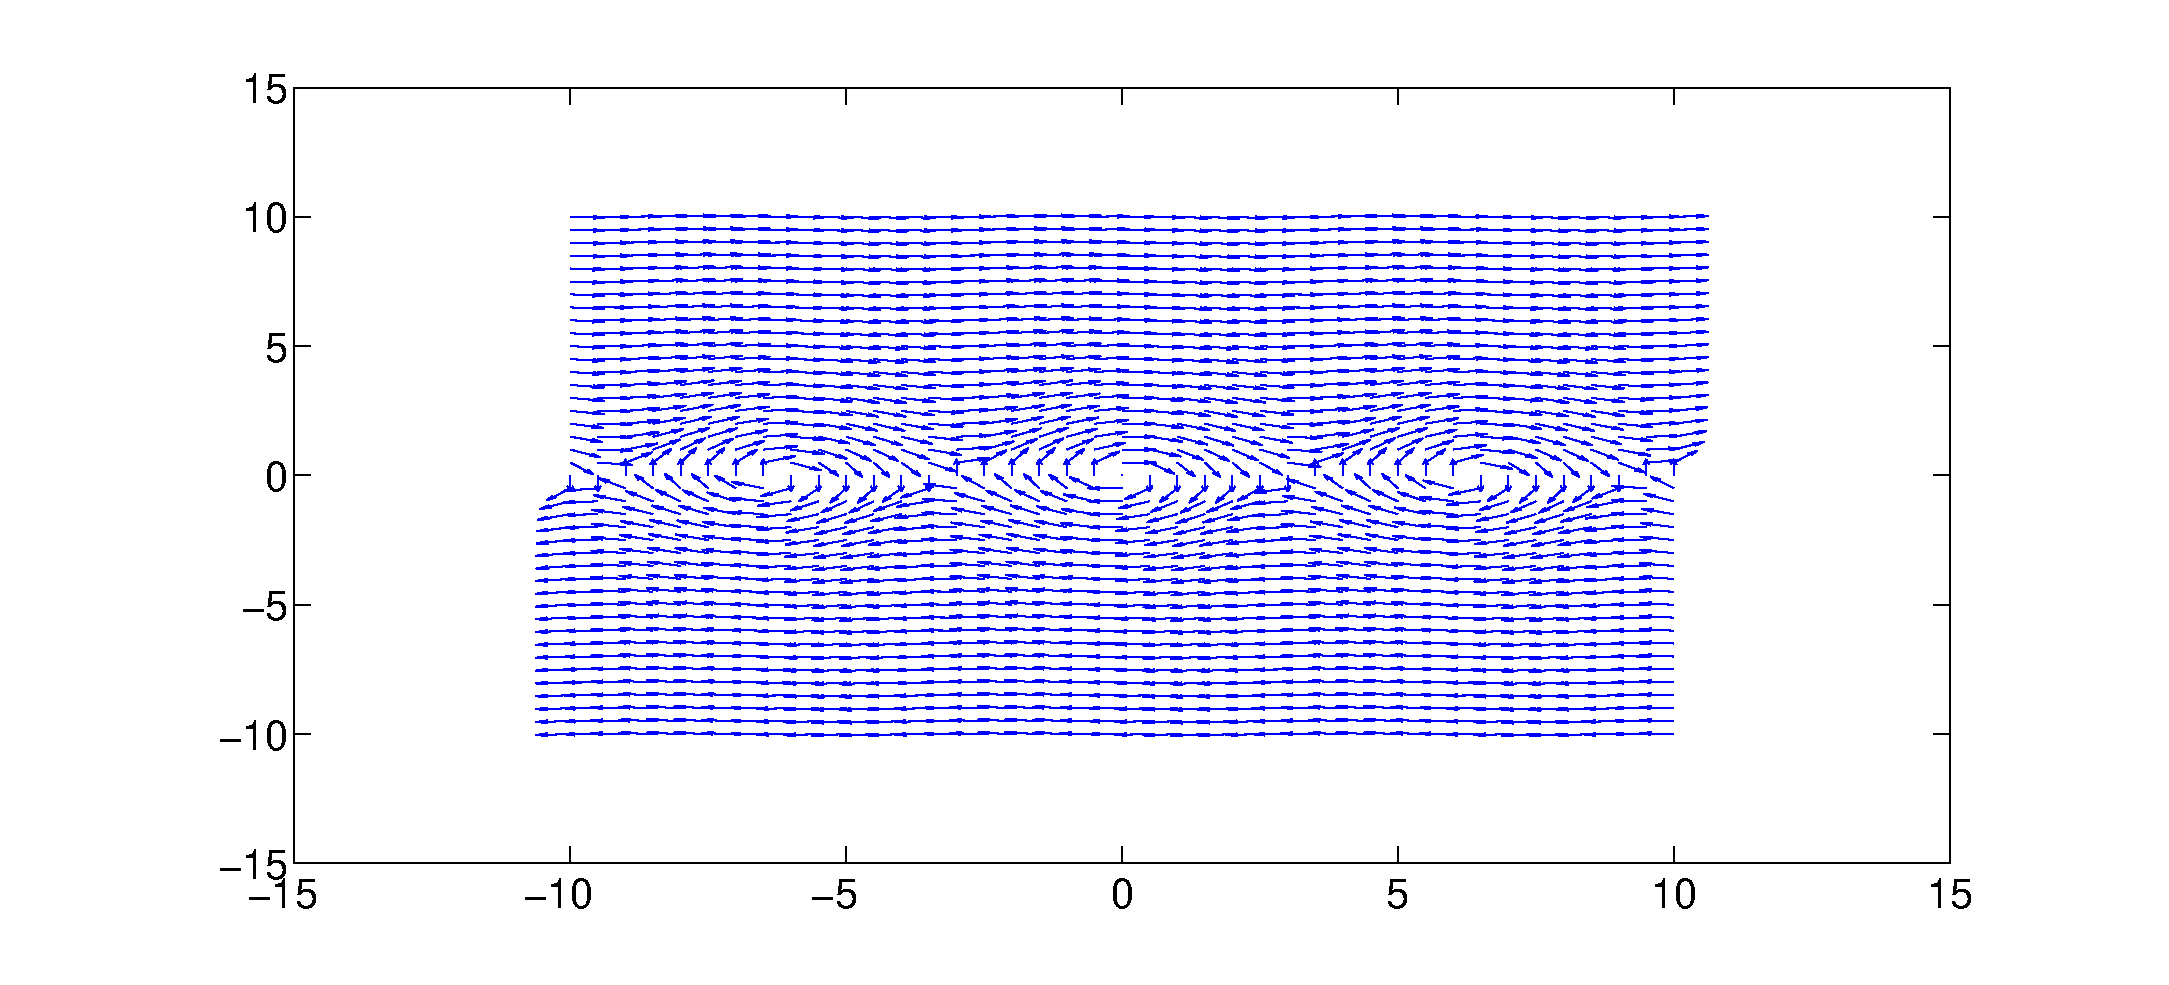
\includegraphics[width=1.0\textwidth]{campo_direzioni_pendolo.eps}
\caption{Campo di direzioni dato da $\mathrm{(SP)}$ con $\omega^2 = 1$.}
\label{T_vs_M}
\end{center}
\end{figure}

Il piano $xy$ è detto anche \emph{piano delle fasi}.  Nel caso $\mathrm{(SP)}$, è facile vedere che i punti di equilibrio (o punti critici) sono dati da
$$
(k\pi,\,0), \qquad k = 0,\, \pm 1,\, \pm 2, \ldots
$$
Pertanto la funzione $x : \mathbb{R} \longrightarrow \mathbb{R}$ definita da
$$
x(t) \doteqdot k\pi, \qquad t \in \mathbb{R}, \; k \text{ fissato in } \mathbb{Z}
$$
è una soluzione di $\mathrm{(EP)}$.

\begin{obs}
Può accadere che due soluzioni si incrocino nel piano $xt$, perché non è detto che abbiano la stessa velocità (hanno derivata prima di $x$ differente).
\begin{center}
\def\svgwidth{8cm}
\input{./04_ODEs/figures/piano_xt_inters.pdf_tex}
\end{center}
Non può invece accadere (per il teorema di esistenza e unicità) che due soluzioni si incontrino in un $t$ finito nel piano delle fasi! A parità di soluzioni, avremmo la stessa velocità! Possono invece toccarsi in un tempo $t$ infinito.
\begin{center}
\def\svgwidth{15cm}
\input{./04_ODEs/figures/piano_xy_inters.pdf_tex}
\end{center}
\end{obs}



\subsubsection{Integrali primi di $\mathrm{(S)}$}
\begin{definition}
Dati $A \subseteq \mathbb{R}^2$ aperto e $f,\,g \in C^1(A)$, una funzione $U \in C^1(A)$ si dice \emph{integrale primo di $\mathrm{(S)}$} nella regione $A$ se
\begin{enumerate}[labelindent=\parindent,leftmargin=*,label=\textnormal{(\roman*)},start=1]
\item $\nabla U(x,\,y) \neq (0,\,0) \qquad \forall (x,\,y) \in A \setminus \lbrace (x,\,y) \in A : f(x,\,y) = g(x,\,y) = 0 \rbrace$
\item Per ogni curva integrale $X : I \longrightarrow \mathbb{R}^2$ di $\mathrm{(S)}$, con $I \subseteq \mathbb{R}$ intervallo, vale
$$
U(X(t)) = U(x(t),\,y(t)) = \text{costante}
$$
\end{enumerate}
\end{definition}


Se in un sistema fisico l'energia si conserva, allora $U$ ha proprio il significato di \emph{energia}. Le curve di livello $\Gamma_c = \lbrace (x,\,y) \in A : U(x,\,y) = c \rbrace$ dove $c \in \mathbb{R}$ costante fissata, si chiamano anche \emph{curve integrali} di $\mathrm{(S)}$.

\begin{obs}[Esercizio 9e, Foglio 7]
Siano $A \subseteq \mathbb{R}^2$ aperto, $f,\,g \in C^1(A)$, e $U \in C^1(A)$ tale che $\nabla U \neq (0,\,0) \qquad \forall (x,\,y) \in A \setminus \lbrace (x,\,y) \in A : f(x,\,y) = g(x,\,y) = 0 \rbrace$. Allora
\begin{center}
$U$ è un integrale primo di $\mathrm{(S)}$
\end{center}
$$
\Updownarrow
$$\vskip 0pt
$$
f(P_0) \frac{\partial U}{\partial x}(P_0) + g(P_0) \frac{\partial U}{\partial y}(P_0) = 0 \qquad P_0 \in A
$$

Tale relazione è facilmente ricavabile osservando che, se $\nabla U \neq (0,\,0)$, la condizione che definisce un integrale primo è
\begin{center}
$\mathrm{(IP)}$
\hfill
$\displaystyle
U(x(t),\,y(t)) = \text{costante}
$
\hfill \null \\
\end{center}
Differenziando $\mathrm{(IP)}$ abbiamo
$$
x'(t_0) \frac{\partial U}{\partial x}(P_0) + y'(t_0) \frac{\partial U}{\partial y}(P_0) = 0 
$$
e, usando $\mathrm{(S)}$,
$$
f(P_0) \frac{\partial U}{\partial x}(P_0) + g(P_0) \frac{\partial U}{\partial y}(P_0) = 0
$$
Questa relazione può anche essere vista nella forma
$$
F(P_0) \bullet \nabla U(P_0) = 0
$$
che appare più intuitiva utilizzando l'interpretazione cinematica. L'orbita della particella è un vincolo dato da $U$, e quindi dal teorema delle funzioni implicite di Dini sappiamo che $\nabla U$ è perpendicolare all'orbita. Poiché $F$, d'altro canto, è tangente all'orbita (rappresenta la velocità!), $\nabla U$ e $F$ sono perpendicolari, ossia il loro prodotto scalare è nullo.
\end{obs}

\begin{thm}
Sia $A \subseteq \mathbb{R}^2$ e sia $U \in C^1(A)$ un integrale primo di $\mathrm{(S)}$. Allora
\begin{enumerate}[labelindent=\parindent,leftmargin=*,label=\textnormal{(\roman*)},start=1]
\item un'orbita $\Gamma \subset A$ di $\mathrm{(S)}$ è contenuta in $\Gamma_c$ per un'opportuna costante $c \in \mathbb{R}$;
\item l'insieme delle curve di livello di $U$ (cioè la famiglia $\Gamma_c = \lbrace (x,\,y) \in A : U(x,\,y) = c \rbrace$ al variare di $c \in \mathbb{R}$) è costituito da un'\emph{unione (disgiunta)} di orbite di $\mathrm{(S)}$.
\end{enumerate}
\end{thm}
\begin{proof}
\mbox{}
\begin{enumerate}[labelindent=\parindent,leftmargin=*,label=\textnormal{(\roman*)},start=1]
\item Sia $\Gamma \subseteq A$ un'orbita di $\mathrm{(S)}$ passante per il punto $(x_0,\,y_0)$, cioè $\Gamma = X(I)$ dove $X : I \longrightarrow \mathbb{R}^2$ è una soluzione di $\mathrm{(S)}$ e $I \subseteq \mathbb{R}$ un intervallo. Fissando $U$ integrale primo di $\mathrm{(S)}$, per definizione vale che
$$
U(X(t)) = U(X(t_0)) = U(x_0,\,y_0) \doteqdot c, \qquad \forall \, t \in I
$$
Quindi $\Gamma \subseteq \Gamma_c$.
\item Sia $c \in \mathbb{R}$ e $\Gamma_c \neq \emptyset$ una curva di livello di $U$. Definiamo
$$
\vartheta_c = \lbrace \Gamma \subseteq \Gamma_c : \Gamma \text{ è un'orbita di } \mathrm{(S)} \rbrace
$$
Dobbiamo provare che
$$
\Gamma_c = \bigcup_{\Gamma \in \vartheta_c} \Gamma
$$
\`{E} banale provare che $\bigcup_{\Gamma \in \vartheta_c} \Gamma \subseteq \Gamma_c$ (già provato al punto $\mathrm{(i)}$). Proviamo quindi che $\Gamma_c \subseteq \bigcup_{\Gamma \in \vartheta_c} \Gamma$. Per il teorema di esistenza e unicità locale di $\mathrm{(PC)}$, otteniamo che $\forall \, (x_0,\,y_0) \in \Gamma_c$, esiste ed è unica un'orbita $\Gamma \in \vartheta_c$ tale che $(x_0,\,y_0) \in \Gamma$. L'unicità ci assicura che l'unione sia disgiunta.
\end{enumerate}
\end{proof}

Ritorniamo al problema di Cauchy da cui siamo partiti
$$
\mathrm{(PCEP)}
\begin{cases}
\; x'' + \omega^2\sin(x) = 0 &\qquad \mathrm{(EP)}\\
\begin{array}{l}
x(t_0) = x_1^0\\
x'(t_0) = x_2^0\\
\end{array}
 &\qquad \mathrm{(CI)}\\
\end{cases}
$$
e al suo sistema associato
$$
\mathrm{(SP)}
\begin{cases}
x' = y\\
y' = -\omega^2\sin(x)\\
\end{cases}
\qquad \qquad
\left(
\begin{array}{rcl}
x(t_0) &=& x_1^0\\
y(t_0) &=& x_2^0\\
\end{array}
\right)
$$
Con l'intento di calcolare l'integrale primo di $\mathrm{(SP)}$ o, equivalentemente, di $\mathrm{(EP)}$, moltiplichiamo ambo i membri di $\mathrm{(EP)}$ per la quantità $ml^2x'$ ottenendo:\footnote{Ricordiamo che $\omega^2 = \dfrac{g}{l}$}
$$
\begin{array}{rcl}
ml^2x'x'' + ml^{\bcancel{2}}x'\dfrac{g}{\bcancel{l}}\sin(x) &=& \\
& \lvert & \\
&=& \dfrac{\mathrm{d}}{\mathrm{d}t}\left( \dfrac{1}{2}ml^2(x')^2 \right) -mlg \dfrac{\mathrm{d}}{\mathrm{d}t}\left( \cos(x) \right)\\
& \lvert & \\
&=& \dfrac{\mathrm{d}}{\mathrm{d}t}\left( \dfrac{1}{2}m(lx')^2 -mgl \cos(x) \right) = 0\\
\end{array}
$$
Definendo le quantità \emph{energia potenziale} ed \emph{energia cinetica} rispettivamente con
$$
E_p \doteqdot mgl(1-\cos(x)), \qquad\qquad E_c \doteqdot \dfrac{1}{2}m(lx')^2
$$
e ponendo
$$
E \doteqdot E_p + E_c
$$
la nostra equazione si riduce a
$$
\dfrac{\mathrm{d}E}{\mathrm{d}t} = 0
\qquad\Longrightarrow\qquad
E = \text{costante}
$$
Abbiamo appena ottenuto la ben nota \emph{legge di conservazione dell'energia}. Utilizzando le $\mathrm{(CI)}$, troviamo
\begin{center}
$\mathrm{(\star)}$
\hfill
$\displaystyle
\dfrac{1}{2}m(lx')^2 - mgl\cos(x) = c_1 = \dfrac{1}{2}m(lx_2^0)^2 - mgl\cos(x_1^0)
$
\hfill \null \\
\end{center}
Dividendo $\mathrm{(\star)}$ per $ml^2$:
$$
\dfrac{1}{2}(x')^2 - \omega^2\cos(x) = c = \dfrac{1}{2}(x_2^0)^2 - \omega^2\cos(x_1^0)
$$
Possiamo quindi definire (ricordando che $y = x'$)
$$
U(x,\,y) = \dfrac{y^2}{2} - \omega^2\cos(x)
$$
\underline{$U$ è un integrale primo di $\mathrm{(SP)}$.} Studiamo ora le sue curve di livello nel piano delle fasi.

Siano $A = \mathbb{R}^2$, $\Gamma_c = \lbrace (x,\,y) \in \mathbb{R}^2 : \dfrac{y^2}{2} - \omega^2\cos(x) = c \rbrace$. Dalla condizione che descrive $\Gamma_c$, abbiamo $c \geq -\omega^2$. Distinguiamo $4$ casi.

\underline{Caso $1$: $c = -\omega^2$}\\
Da $U$, otteniamo
$$
y^2 = 2\omega^2(-1+cos(x))
\qquad\Longleftrightarrow\qquad
(x,\,y) = (2n\pi,\,0) \quad n \in \mathbb{Z}
$$
Dunque $\Gamma_c = \lbrace (2n\pi,\,0) : n \in \mathbb{Z} \rbrace$. Nel piano delle fasi:
\begin{center}
\def\svgwidth{8cm}
\input{./04_ODEs/figures/pendolo_1_fasi.pdf_tex}
\end{center}

\underline{Caso $2$: $-\omega^2 < c < \omega^2$}\\
Da $U$, otteniamo
$$
y^2 = 2(c+\omega^2\cos(x))
\qquad\Longrightarrow\qquad
c+\omega^2\cos(x) \geq 0
\qquad\Longleftrightarrow\qquad
\cos(x) \geq -\dfrac{c}{\omega^2}
$$
Ora, esistono $x_1,\,x_2 \in (-\pi,\,\pi)$ con $-\pi < x_1 < 0 < x_1 < \pi$ tali che
$$
\cos(x) \geq -\dfrac{c}{\omega^2}
\qquad\Longleftrightarrow\qquad
x_1 \leq x \leq x_2
$$
\begin{center}
\def\svgwidth{8cm}
\input{./04_ODEs/figures/pendolo_2_fasi.pdf_tex}
\end{center}

\underline{Caso $3$: $c = \omega^2$}\\
Da $U$, otteniamo
$$
y^2 = 2\omega^2(1+\cos(x))
\qquad\Longleftrightarrow\qquad
\Gamma_c = \lbrace (x,\, \pm \sqrt{2}\omega\sqrt{1+\cos(x)}) : x \in \mathbb{R} \rbrace
$$
Osserviamo che
$$
((2n+1)\pi,\,0) \in \Gamma_c \qquad \forall \, n \in \mathbb{Z}
$$
\begin{center}
\def\svgwidth{8cm}
\input{./04_ODEs/figures/pendolo_3_fasi.pdf_tex}
\end{center}

\underline{Caso $4$: $c > \omega^2$}\\
Da $U$, otteniamo
$$
y^2 = 2\omega^2(c+\cos(x))
\qquad\Longrightarrow\qquad
c+\omega^2\cos(x) > 0 \qquad \forall x \in \mathbb{R}
$$
$$
\Gamma_c = \lbrace (x,\, \pm \sqrt{2}\sqrt{c+\omega^2\cos(x)}) : x \in \mathbb{R} \rbrace
$$
\begin{center}
\def\svgwidth{8cm}
\input{./04_ODEs/figures/pendolo_4_fasi.pdf_tex}
\end{center}

Vediamo ora i possibili grafici delle soluzioni nel piano $tx$ per ogni caso.

\underline{Caso $1$: $c = -\omega^2$}\\
Le soluzioni sono della forma
$$
x(t) = 2n\pi \qquad n \in \mathbb{Z}
$$
In questo caso, abbiamo le cosiddette \emph{soluzioni di equilibrio}:
\begin{center}
\def\svgwidth{8cm}
\input{./04_ODEs/figures/pendolo_1_soluz.pdf_tex}
\end{center}

\underline{Caso $2$: $-\omega^2 < c < \omega^2$}\\
La forma della soluzione è nella figura sottostante. Ma, a questo punto, sorge spontanea la domanda: la soluzione è \emph{periodica}? Cioè, $\exists \, \text{\LARGE $\tau$} \in \mathbb{R}$ ed esiste $x_{\max} : \mathbb{R} \longrightarrow \mathbb{R}$ soluzione di $\mathrm{(EP)}$ tale che
$$
x(t+\text{\LARGE $\tau$}) \qquad \forall \, t \in \mathbb{R}?
$$
Si può provare che, fissate le condizioni iniziali per cui
$$
\begin{cases}
x'' + \omega^2\sin(x) = 0\\
x(t_0) = x_1^0, \quad x'(t_0) = x_2^0
\end{cases}
$$
allora $I_{\max} \equiv \mathbb{R}$ e $x_{\max}$ è periodica.
\begin{center}
\def\svgwidth{8cm}
\input{./04_ODEs/figures/pendolo_2_soluz.pdf_tex}
\end{center}

\underline{Caso $3$: $c = \omega^2$}\\
In questo caso, abbiamo soluzioni di \emph{equilibrio} più soluzioni che \emph{connettono} stati di equilibrio.
\begin{center}
\def\svgwidth{8cm}
\input{./04_ODEs/figures/pendolo_3_soluz.pdf_tex}
\end{center}

\underline{Caso $4$: $c > \omega^2$}\\
Questo è il caso delle cosiddette \emph{soluzioni vorticose}, che hanno un andamento strettamente crescente o decrescente, in quanto
$$
x' = \sqrt{2(c+\omega^2\cos(x))} > 0
$$
\begin{center}
\def\svgwidth{8cm}
\input{./04_ODEs/figures/pendolo_4_soluz.pdf_tex}
\end{center}

Riprendiamo ora il caso $2$, in cui ci eravamo chiesti se la soluzione trovata si potesse ``estendere'' ad una soluzione periodica. Ricordiamo innanzitutto la definizione.

\begin{definition}
Una soluzione $X = (x,\,y) : \mathbb{R} \longrightarrow \mathbb{R}^2$ di $\mathrm{(S)}$ si dice \emph{periodica} se $\exists \, \text{\LARGE $\tau$} \in \mathbb{R}$  tale che
$$
X(t+\text{\LARGE $\tau$}) \qquad \forall \, t \in \mathbb{R}
$$
\end{definition}

La periodicità della soluzione del caso $2$ ci è garantita dal seguente teorema.

\begin{thm}
Sia $A \subseteq \mathbb{R}^2$ aperto e sia $U \in C^1(A)$ un integrale primo di $\mathrm{(S)}$. Definiamo, per un dato $c>0$, 
$$
\Gamma_c \doteqdot \lbrace (x,\,y) \in \mathbb{R}^2 : U(x,\,y) = c \rbrace
$$
e supponiamo che
\begin{enumerate}[labelindent=\parindent,leftmargin=*,label=\textnormal{(\roman*)},start=1]
\item $\Gamma_c$ è una curva \emph{chiusa, regolare e semplice}, cioè, per definizione,
	\begin{itemize}
	\item $\exists \, \varphi : [a,\,b] \longrightarrow A$ di classe $C^1(A)$ e $\varphi'(s) \neq (0,\,0) \quad \forall \, s \in [a,\,b]$ \emph{(regolare)}
	\item $\varphi(a) = \varphi(b)$ \emph{(chiusa)}
	\item $\varphi : [a,\,b] \longrightarrow A$ è iniettiva \emph{(semplice)}	
	\end{itemize}
\item $\Gamma_c$ non contiene punti di equilibrio di $\mathrm{(S)}$
\end{enumerate}
Allora $\Gamma_c$ è un'orbita periodica, cioè, per definizione, esiste $X: \mathbb{R} \longrightarrow \mathbb{R}^2$ soluzione di $\mathrm{(S)}$ periodica e $\Gamma_c = X(\mathbb{R})$.
\end{thm}



